\input{head.inc}
  
% Präambelbefehle für die Präsentation
\title[TET: Elektromagnetische Wellen IV - Polarisation Ebenen Wellen]{Elektromagnetische Wellen IV - Polarisation Ebenen Wellen}

\begin{document}
% 
% Frontmatter 
% 
%%%%%%%%%%%%%%%%%%%%%%%%%%%%%%%%%%%%%%%%%%%%%%%%%%%%%%%%%%%%%%%%%%%%%%%%%%%%%%%%%%%%%%%%%%%%%%%%%%%%%%%%%%%%%%%%%%%%%%%%%%%%% 

%% inserts the title page and the table of contents
\maketitle

% 
% Content 
% 
%%%%%%%%%%%%%%%%%%%%%%%%%%%%%%%%%%%%%%%%%%%%%%%%%%%%%%%%%%%%%%%%%%%%%%%%%%%%%%%%%%%%%%%%%%%%%%%%%%%%%%%%%%%%%%%%%%%%%%%%%%%%% 
\section{Elektromagnetische Wellen IV - Polarisation Ebenen Wellen}

\begin{frame}
  \frametitle{Ausgangspunkt}
  \begin{itemize}[<+->]
  \item Wir betrachten \alert{monochromatische ebene Wellen}, die in \(+z\)-Richtung propagieren
\begin{align*}
\EFeld[uv] &= \left( \EFeld[u]_{0x}\einheitsvek{x} + \EFeld[u]_{0y}\einheitsvek{y}\right)\euler^{\komplex ( \omega t - \Wellenzahl z)} &
\BFeld[uv] &= \frac{1}{\Geschwindigkeit_{\mathrm{p}}}\left(-\EFeld[u]_{0y}\einheitsvek{x} +\EFeld[u]_{0x}\einheitsvek{y}\right) \euler^{\komplex(\omega t - \Wellenzahl z)} & \Geschwindigkeit_{\mathrm{p}}= \frac{\omega}{k} \stackrel{\text{hier}}{=} \Geschwindigkeit_{\mathrm{c}}
\end{align*}
\item Hierbei sind: 
\begin{align*}
\EFeld[u]_{0x} &= \vert \EFeld[u]_{0x} \vert \cdot \euler^{\komplex \varphi_x} \text{ komplexe Komponente in \(x\)-Richtung bei \(t=0, z=0\)}\\
\EFeld[u]_{0y} &= \vert \EFeld[u]_{0y} \vert \cdot \euler^{\komplex (\varphi_x+ \delta)} \text{ dito für \(y\)-Komponente}\\
\EFeld[v] (\Ortsr[v], t) &= \real{\EFeld[u](\Ortsr[v], t)} = \EFeld_x \einheitsvek{x} + \EFeld_y \einheitsvek{y} \text{ Physikalische Lösung}\\
\EFeld_x &= \vert \EFeld[u]_{0x} \vert \cos(\omega t - \Wellenzahl z + \varphi_x )\\
\EFeld_y &= \vert \EFeld[u]_{0y} \vert \cos(\omega t - \Wellenzahl z + \varphi_x +\delta)\\
\varphi_x &: \text{ gemeinsamer Phasenwinkel \(\to\) relativ unwichtig}\\
\delta &: \text{ relative Phase \(\to\) \alert{Fallunterscheidung}}
\end{align*}
\item Fallunterscheidung in drei Spezialfälle (sowie: \(\delta\) und \(\vert \EFeld[u]_{0x} \vert, \vert \EFeld[u]_{0y} \vert\) beliebig):
  \begin{itemize}[<+->]
  \item \(\delta = 0, \pm \pi , \pm 2\pi, \ldots\)
  \item \(  \delta = \pm \frac{\pi}{2}, \pm \frac{3\pi}{2},\ldots \quad ;\quad\vert \EFeld[u]_{0x} \vert = \vert \EFeld[u]_{0y} \vert = \hat{\EFeld} \)
  \item \( \delta = \pm \frac{\pi}{2}, \pm \frac{3\pi}{2},\ldots \quad ;\quad\vert \EFeld[u]_{0x} \vert \neq \vert \EFeld[u]_{0y} \vert \)
  \end{itemize}
\end{itemize}
\ 
\end{frame}


\begin{frame}
  \frametitle{1. Fall: Lineare Polarisation}
  \begin{itemize}[<+->]
  \item Wir betrachten: \(\delta = z \cdot \pi ,\quad z \in \IZ\quad\rightarrow\quad \delta = \textcolor{green!70}{0}, \textcolor{red}{\pm \pi} , \textcolor{green!70}{\pm 2\pi}, \ldots\)
 \item Für den Cosinus gilt die Beziehung  
    \begin{align*}
\begin{split}
\cos ( \alpha + \delta ) = \cpm \cos \alpha \quad;\quad &\textcolor{green!70}{+} : \pointspace 0,\pm 2\pi, \pm 4\pi, \ldots\\
& \textcolor{red}{-} : \pointspace \pm \pi, \pm 3\pi, \ldots
\end{split}
\end{align*}
\item Hiermit ergibt sich für das elektrische Feld
\begin{align*}
  \Rightarrow \EFeld[v]&= \underbrace{(\vert \EFeld[u]_{0x} \vert \einheitsvek{x} \cpm \vert \EFeld[u]_{0y}\vert \einheitsvek{y})}_{\substack{\text{fester Vektor, orts- und}\\ \text{zeitunabhängig}}} \cos (\omega t - \Wellenzahl z + \varphi_x)\\
  &= \hat{\EFeld}\cdot \einheitsvek{\EFeld}\cos (\omega t - \Wellenzahl z + \varphi_x ) \text{ \(\to\) \alert{linear Polarisiert}}\\
  \hat{\EFeld} &= \vert \EFeld[v] \vert = \sqrt{\vert \EFeld[u]_{0x} \vert ^2 + \vert \EFeld[u]_{0y} \vert ^2}
\end{align*}
\item \alert{Polarisationswinkel}
  \begin{columns}
    \begin{column}{.2\linewidth}
      \hspace*{1cm}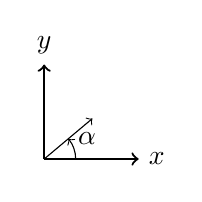
\begin{tikzpicture}[scale=0.4]
	% Achsen zeichnen
	\draw[->,thick] (0,0) -- (3,0) node[right] {$x$};
	\draw[->,thick] (0,0) -- (0,3) node[above] {$y$};
	%Plot
    \draw[->] (0,0) --(40:2) node[right] {$\einheitsvek{\EFeld}$};
    \draw[->] (0:1)arc(0:40:1) node[right] {$\alpha$};
\end{tikzpicture}
      \end{column}
      \begin{column}{.2\linewidth}
        \(\tan \alpha = \cpm \dfrac{|\EFeld[u]_{0y}|}{|\EFeld[u]_{0x}|}\)
      \end{column}
      \begin{column}{.6\linewidth}
Allgemeinen Lösung: Überlagerung zweier linear polarisierter Beiträge in \(x\)- bzw. \(y\)-Richtung.\\
\(\Rightarrow\) \alert{Jede beliebige Polarisation ist darstellbar als Überlagerung zweier zueinander senkrechter linearer Polarisationen!}
\end{column}
    \end{columns}
  \end{itemize}
  \ 
\end{frame}

\begin{frame}
  \frametitle{2. Fall: Zirkulare Polarisation}
  \begin{itemize}[<+->]
  \item Wir betrachten: \(\delta = (2m+1) \frac{\pi}{2}, \quad m \in \IZ , \quad\delta = \pm \frac{\pi}{2}, \pm \frac{3\pi}{2},\ldots \quad ;\quad\vert \EFeld_{0x} \vert = \vert \EFeld_{0y} \vert = \hat{\EFeld} \)
  \item Für den Cosinus gilt die Beziehung
    \begin{align*}
\begin{split}
 \cos ( \alpha + \delta ) = \cmp \sin \alpha \quad;\quad &\textcolor{red}{+} : \pointspace -\frac{\pi}{2} + m (2\pi) \quad\textcolor{green!70}{-} : \pointspace  +\frac{\pi}{2} + m (2 \pi), \quad m \in \IZ
\end{split}
\end{align*}
\item Hiermit ergibt sich für das elektrische Feld
\begin{align*}
  \EFeld[v] &= \hat{\EFeld}(\cos(\omega t - \Wellenzahl z + \varphi_x)\einheitsvek{x} \cmp \sin (\omega t - \Wellenzahl z + \varphi_x)\einheitsvek{y})
\end{align*}
\item Für festes \(z\) oder \(t\): Kreis mit Radius \(\hat{\EFeld}\)
  \(\to\) \alert{Zirkulare Polarisation}
  \medskip
  
  \begin{columns}
    \begin{column}{.50\linewidth}
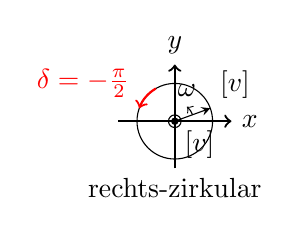
\begin{tikzpicture}[scale=0.4]
	% Achsen zeichnen
	\draw[->,thick] (-1.8,0) -- (1.8,0) node[right] {$x$};
	\draw[->,thick] (0,-1.5) -- (0,1.8) node[above] {$y$};
	%Plot
	%\draw[style=dashed] (-1.27,-1.05) rectangle (1.27,1.05);
	\draw (0, 0) circle (1.2);
	\draw (0, 0) circle (.2);
	\draw[fill=black] (0, 0) circle (.1);
	\draw (0,0) node[below right] {$\Wellenzahl[v]$};
	\draw[->,>=stealth] (0,0)--(20:1.2) node[above right] {$\EFeld[v]$};
	\draw[->] (20:.6) arc (20:50:.6) node [above] {$\omega$};
	\draw [->,thick,color=red] (120:1.2) arc (120:160:1.2) node[above left] {$\delta = -\frac{\pi}{2}$};
	\draw (0,-1.5) node[below]{rechts-zirkular}; 
\end{tikzpicture}
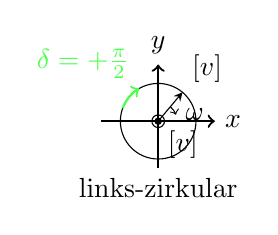
\begin{tikzpicture}[scale=0.4]
	% Achsen zeichnen
	\draw[->,thick] (-1.8,0) -- (1.8,0) node[right] {$x$};
	\draw[->,thick] (0,-1.5) -- (0,1.8) node[above] {$y$};
	%Plot
	%\draw[style=dashed] (-1.27,-1.05) rectangle (1.27,1.05);
	\draw (0, 0) circle (1.2);
	\draw (0, 0) circle (.2);
	\draw[fill=black] (0, 0) circle (.1);
	\draw (0,0) node[below right] {$\Wellenzahl[v]$};
	\draw[->,>=stealth] (0,0)--(50:1.2) node[above right] {$\EFeld[v]$};
	\draw[->] (50:.6) arc (50:20:.6) node [right] {$\omega$};
	\draw [->,thick,color=green!70] (160:1.2) arc (160:120:1.2) node[above left] {$\delta = +\frac{\pi}{2}$};
	\draw (0,-1.5) node[below]{links-zirkular}; 
      \end{tikzpicture}
    \end{column}
    \begin{column}{.41\linewidth}
      \begin{itemize}[<+->]
      \item \alert{Überlagerung} zweier links und rechts umlaufenden zirkular polarisierter Wellen (unterschiedlicher Amplitude) ergibt wieder eine \alert{beliebig polarisierte Welle.}
      \item gleiche Amplitude \(\to\) linear polarisiert
      \end{itemize}
    \end{column}
    \end{columns}
  \end{itemize}
  \ 
\end{frame}


\begin{frame}
  \frametitle{3. Fall: Elliptische Polarisation}
  \begin{itemize}[<+->]
  \item Wir betrachten: \(\delta = (2m+1) \frac{\pi}{2}, \quad m \in \IZ , \quad\delta = \pm \frac{\pi}{2}, \pm \frac{3\pi}{2},\ldots \quad ;\quad\vert \EFeld_{0x} \vert \neq \vert \EFeld_{0y} \vert  \)
\item Analog zur zirkularen Polarisation folgt für das elektrische Feld
    \begin{align*}
\EFeld_x &= \vert \EFeld_{0x} \vert \cos (\omega t - \Wellenzahl \Ortsr + \varphi_x)\\
\EFeld_y &= \cmp \vert \EFeld_{0y} \vert \sin (\omega t - \Wellenzahl \Ortsr + \varphi_x)\\
\Rightarrow &\left[ \frac{\EFeld_x}{\vert \EFeld[u]_{0x}\vert}\right]^2+\left[\frac{\EFeld_y}{\vert \EFeld[u]_{0y}\vert}\right]^2 = 1\quad\text{Ellipse, Halbachsen }\vert \EFeld_{0x} \vert , \vert \EFeld_{0y} \vert
\end{align*}
\item \alert{Elliptisch polarisierte Wellen} (rechts und links umlaufend)

  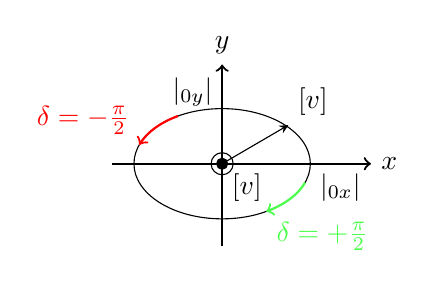
\begin{tikzpicture}[scale=0.7]
	% Achsen zeichnen
	\draw[->,thick] (-2,0) -- (2.7,0) node[right] {$x$};
	\draw[->,thick] (0,-1.5) -- (0,1.8) node[above] {$y$};
	%Plot
	%\draw[style=dashed] (-1.27,-1.05) rectangle (1.27,1.05);
	\draw (0, 0) ellipse (1.6 and 1);
	\draw(1.6,0) node[below right] {$|\EFeld_{0x}|$} ;
	\draw(0,1.3) node[left] {$|\EFeld_{0y}|$} ;
	\draw[->,>=stealth] (0,0)--(1.2,0.7) node[above right] {$\EFeld[v]$};
	%\draw[->,color=green] (40:1) arc (40:160:1.3);
	\draw [->,thick,color=green!70] plot[domain=340:300] ({cos(\x)*1.6},{sin(\x)}) node[below right] {$\delta = +\frac{\pi}{2}$};
	\draw [->,thick,color=red] plot[domain=120:160] ({cos(\x)*1.6},{sin(\x)}) node[above left] {$\delta = -\frac{\pi}{2}$};
	\draw (0, 0) circle (.2);
	\draw[fill=black] (0, 0) circle (.1);
	\draw (0,0) node[below right] {$\Wellenzahl[v]$};
\end{tikzpicture}
\end{itemize}
\end{frame}


\begin{frame}
  \frametitle{4. Fall: keine Einschränkungen}
  \begin{itemize}[<+->]
  \item Keine Einschränkungen für \(\delta\) und \(\vert \EFeld_{0x} \vert\) bzw. \(\vert \EFeld_{0y} \vert  \)
  \item Analog zur zirkularen Polarisation folgt ohne weitere Herleitung:
    \begin{itemize}[<+->]
    \item Ebenfalls \alert{elliptisch polarisiert}
      \item aber die Halbachsen sind gegen das \(x\)-\(y\)-System gedreht
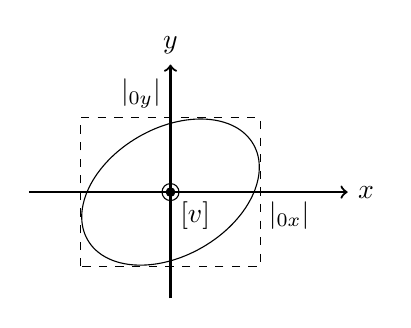
\begin{tikzpicture}[scale=0.9]
	% Achsen zeichnen
	\draw[->,thick] (-2,0) -- (2.5,0) node[right] {$x$};
	\draw[->,thick] (0,-1.5) -- (0,1.8) node[above] {$y$};
	%Plot
	\draw[style=dashed] (-1.27,-1.05) rectangle (1.27,1.05);
	\draw[rotate=30] (0, 0) ellipse (1.35 and 0.9);
	\draw(1.25,0) node[below right] {$|\EFeld_{0x}|$} ;
	\draw(0,1.05) node[above left] {$|\EFeld_{0y}|$} ;
	\draw (0, 0) circle (.12);
	\draw[fill=black] (0, 0) circle (.06);
	\draw (0,0) node[below right] {$\Wellenzahl[v]$};
\end{tikzpicture}
      \end{itemize}

\item Eine beliebige Polarisation lässt sich zusammensetzen aus
\begin{itemize}
\item 2 linear polarisierte Wellen, zueinander $\bot$
\item 2 zirkular polarisierte Wellen, entgegenlaufend
\end{itemize}
\end{itemize}
\end{frame}

\begin{frame}
  \frametitle{Visualisierung}
  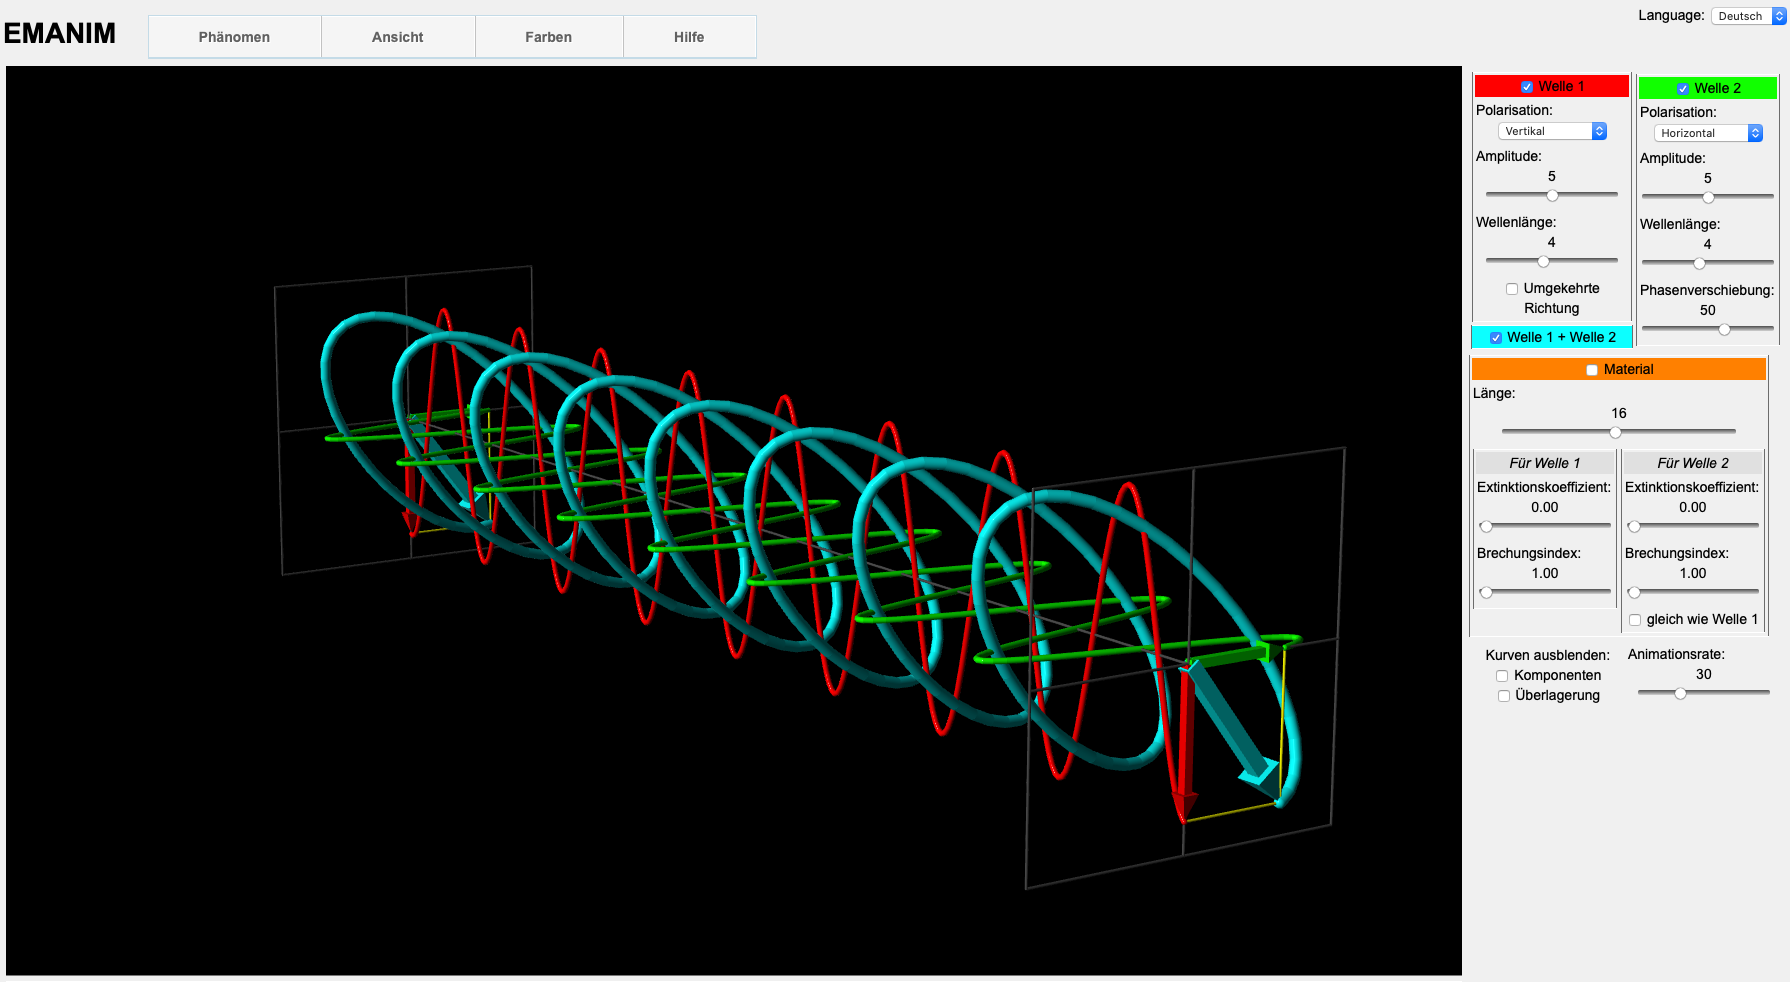
\includegraphics[width=\linewidth]{EMANIM}
  
  Szilágyi, András (2019): \enquote{EMANIM: Interactive visualization of electromagnetic waves}. Web application available at URL \url{https://emanim.szialab.org}
\end{frame}



\input{finalframe.inc}
   
\end{document}